\chapter{\textbf{Metodologia de Pesquisa}} % Este comando é utilizado para criar capítulos
\sloppy % Corrige estouro de linhas

\section{Aplicativo}

O escopo da aplicação foi definido para contemplar uma base de dados já existente de um sistema de gerenciamento escolar já implantado em um município, o qual cedeu o acesso à mesma para utilização na construção do software. Após a construção, o software ficará disponível para utilização por parte da população do município, bem como toda a sua codificação.

Para a construção do mesmo, foi utilizado como referência de metodologia de desenvolvimento o modelo aplicado na disciplina de Laboratório de Engenharia de Software do curso de Sistemas de Informação do Ifes Campus Cachoeiro, baseado no \textit{Rational Unified Process} (RUP), representado na figura \ref{figura:rup}. 

\begin{figure}[H]
	\caption{Processo de desenvolvimento de \textit{software} baseado no RUP.}
	\centering % para centralizarmos a figura
	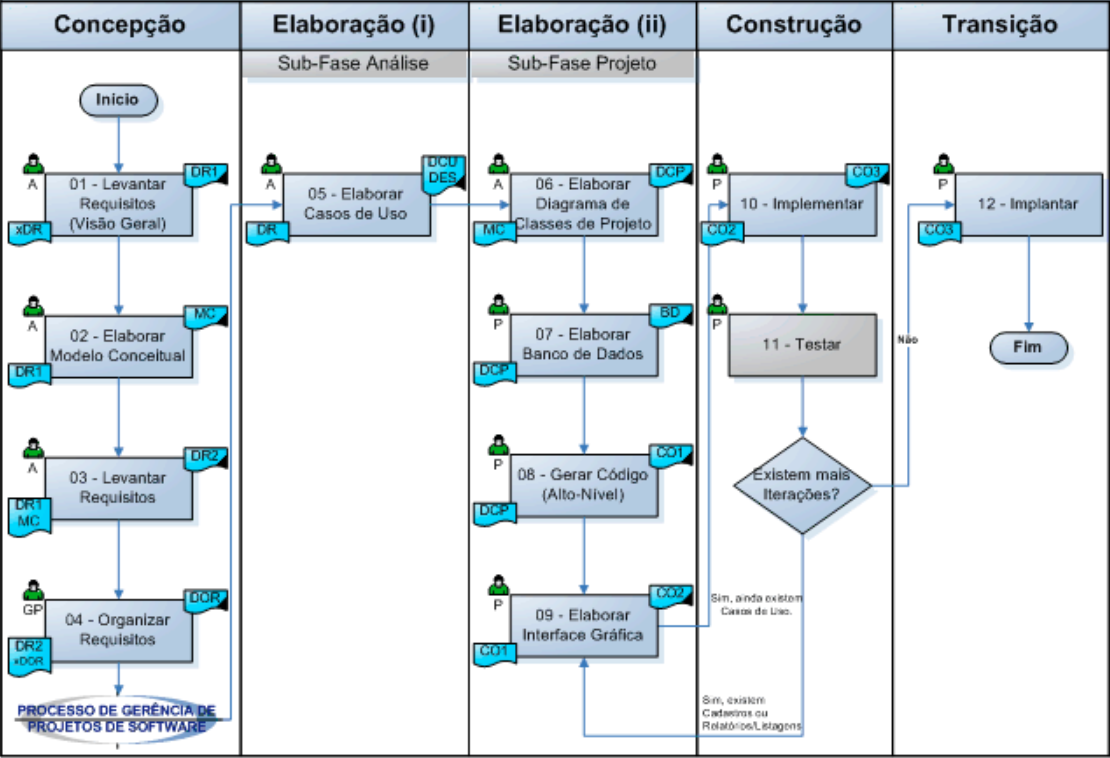
\includegraphics[width=16cm]{resources/pds_rup.png} % leia abaixo
	\label{figura:rup}
	\captionsetup{singlelinecheck = false, format= hang, justification=raggedright, labelsep=space, width=16cm}
	\caption*{\footnotesize Fonte: \citeonline{rupLes}.}
\end{figure}

Para tal, os seguintes passos descritos no modelo (figura \ref{figura:rup}) foram executados para a elaboração do \textit{sofware}:

\begin{enumerate}
   \item Levantar Requisitos (Visão Geral): identificar descrever de forma geral o funcionamento do aplicativo e suas principais funções;
   \item Elaborar modelo conceitual: identificar classes e relacionamentos concernentes ao domínio (nesta fase não se faz necessário a inclusão dos atributos nas classes);
   \item Levantar Requisitos: elaborar documento de requisitos contendo o detalhamento de todas as funcionalidades do aplicativo;
   \item Organizar Requisitos: elaborar documento de organização de requisitos separando todos os requisitos em processos de negócios e relatórios/listagens;
   \item Elaborar banco de dados: 
   \item Elaborar interface gráfica: estruturar todas as telas do aplicativo;
   \item Implementar: codificar as classes necessárias para implementação das funcionalidades de processos de negócio e listagens;
   \item Testar: realizar testes de todas as funcionalidades implementadas;
   \item Implantar: gerar o arquivo instalável do aplicativo (APK) e instalar o \textit{webservice} no servidor de produção;
\end{enumerate}

\section{Módulo de Recomendação baseado em Redes Neurais}

Considerando as áreas de conhecimento definidas pelo Novo Ensino Médio \cite{lei13415}, foi realizado a construção de um módulo de recomendação aptidão do aluno. Para tanto, foram realizadas as seguintes etapas no processo de desenvolvimento:

\begin{enumerate}
   \item Selecionar variáveis para o treinamento da rede;
   \item Preparar o arquivo de treinamento com base nas variáveis escolhidas;
   \item Realizar o treinamento da rede;
   \item Implementar o módulo junto ao web service do aplicativo;
\end{enumerate}

Para a construção do módulo de recomendação do aplicativo foi utilizado a biblioteca Weka para realizar o treinamento da rede e extrair os resultados do mesmo. Para tanto, a biblioteca utiliza um arquivo do tipo ARFF para descrever os os atributos, as possibilidades de classificação, e os respectivos exemplos de classificação utilizados no treinamento em questão. Sua estrutura básica é representada na figura \ref{figura:arff}.

\begin{figure}[H]
	\caption{Sintaxe básica de um arquivo de treinamento utilizado pelo Weka.}
	\centering % para centralizarmos a figura
	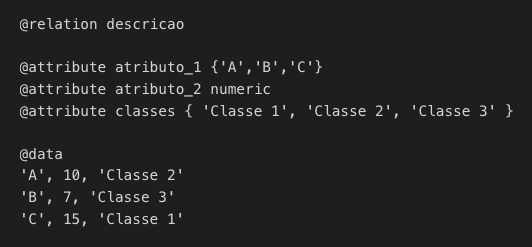
\includegraphics[width=12cm]{resources/arff.png} % leia abaixo
	\label{figura:arff}
	\captionsetup{singlelinecheck = false, format= hang, justification=raggedright, labelsep=space, width=12cm}
	\caption*{\footnotesize Fonte: O Autor.}
\end{figure}

\section{Ambiente de desenvolvimento}

As seguintes ferramentas e \textit{softwares} foram utilizados no processo de desenvolvimento:

\begin{itemize}
    \item Java SE \textit{Development Kit} (versão 8 update 221);
    \item Ionic \textit{Framework} (versão 4);
    \item Servidor Web Payara (versão 5.191);
    \item Netbeans IDE (versão 11.1);
    \item Visual Studio Code (versão 1.39.1);
    \item Postman (versão 7.2);
\end{itemize}

\section{Arquitetura da Aplicação}

Toda a aplicação foi construída baseado na arquitetura REST \cite{fielding2000}, seguindo a estrutura representada na figura \ref{figura:arqu_basica}. Neste modelo, é construído uma API REST que busca as informações referentes aos alunos na base de dados, trata os mesmos, e retorna no formato JSON para a aplicação instalada nos \textit{smartphones}, que poderão utilizar tanto o sistema Android, quanto IOS.

\begin{figure}[H]
	\caption{Arquitetura básica da Aplicação.}
	\centering % para centralizarmos a figura
	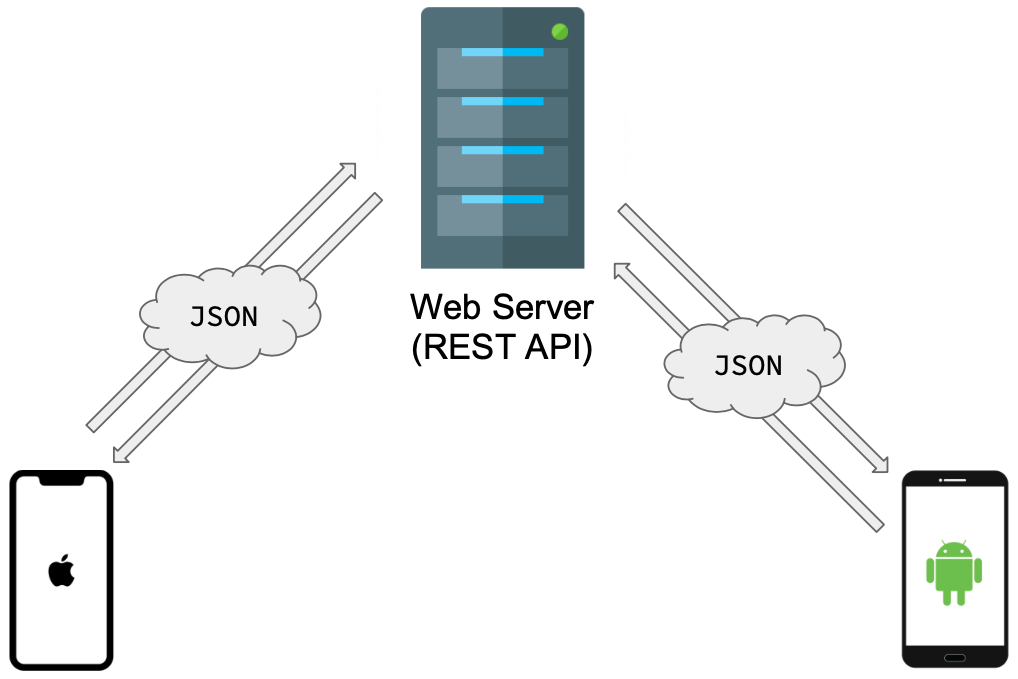
\includegraphics[width=12cm]{resources/esquema_web_service.png} % leia abaixo
	\label{figura:arqu_basica}
	\captionsetup{singlelinecheck = false, format= hang, justification=raggedright, labelsep=space, width=12cm}
	\caption*{\footnotesize Fonte: O Autor.}
\end{figure}